\chapter{Workflows for post-editing projects -- which decisions have to be taken?}\label{sec:8}

    \objectives{
        You will learn...
        \begin{itemize}
            \item which aspects are important, when deciding whether machine translation and post-editing can be used for a translation job,
            \item how to assess these aspects,
            \item who is responsible for these decisions.
        \end{itemize}
        }

\vspace{\baselineskip}

According to \citet{hofmann2012prozessgestutztes}, the translation process consists of three steps: translation preparation, translation, and translation post-processing. \citet{hor_chancen_2020} assigned the same steps to the PE process in her MA thesis. While the translation is performed by the MT system and the translation post-processing by the post-editor,\footnote{Consider the changing balance: While in translation processes, the main focus is on the second step (translation), the main focus in PE shifts towards the last step (translation post processing).} the PE preparation has to be conducted by the client, the project manager, or the post-editor him/herself. In this section, we will concentrate on this preparatory step where different decisions have to be made, most importantly whether MT can be used and to what extent PE is needed. The standard ISO 18587 on PE already mentions this preparation step in the PE process: “[b]esides the general commercial aspects, there is also the question of whether the source text is actually suitable for MT” \citep[150]{wallberg_iso_2017}. However, the standard does not explain, how this question is answered. Further, we think it is not only the source text, but also other factors that contribute to the decision whether or not the project is suitable for PE and what PE guidelines are needed. Therefore, we want to present different criteria that can help customers and other decision makers, like project managers, decide whether MT can be implemented in the translation process, focusing first on the source text (\sectref{sec:8:1}), then on the choice of MT system (\sectref{sec:8:2}), and finally on the target text (\sectref{sec:8:3}). 

\section{Text types, risk considerations, and data security}\label{sec:8:1}

First, as already advised by the PE standard (\sectref{sec:4:2}), we want to take a closer look at the source text. As you will remember, we have talked about the single components in previous chapters. Whether a source text is suitable for MT can be determined by its text type (\sectref{sec:5}), the risks associated with the text type (\sectref{sec:7:1}), and how sensitive the content(s) of the text(s) are (\sectref{sec:7:2}).

As discussed in \sectref{sec:5}, it is usually advisable to use MT for text types that are not very creative, contain redundancies, and may have been created using specific guidelines and rules or even using a controlled language. Very creative texts such as different forms of literature, marketing texts, or slogans should generally be translated from scratch, because they also need creative translations that might differ greatly from the source text (e.g. in \textit{transcreation} jobs, \citealt{pedersen2014exploring}). Here, we would also like to mention that each text has individual characteristics, even if they belong to the same text type. Hence, texts from the same/similar text types might be more or less suitable for MT.

MT output is often quite linear to the source text, which is often not desirable in creative texts. Accordingly, the PE effort might be too high. Further, it could be argued that PE might suppress creative translations. However, \citet[113]{o2012translation} claims that “this [editing as a less creative task] is certainly open to debate – can we really argue that improving or correcting what an author has written is ‘less creative’ than translating another author’s words?” Restricted texts, like most domain-specific communication on the other hand, are in general more suitable for MT because linearity and similarity to the source text is acceptable and often even favoured. Hence, the question at the beginning of the potential PE job is whether MT can be used at all in the specific situation. Therefore, it must be assessed whether the text is suited for MT. As a rough rule of thumb, we suggest that if the texts seem suitable for processing with the help of  translation memory software, they can also be processed by MT \citep[221--224]{arnhold_maschinelle_2017}. In recent years, the borders have become more and more blurry and it is becoming difficult to tell by the text type alone whether or not to use MT. At this point, we might already have to consider the purpose of the translation. To summarise: If we want to translate poems for publication, we probably should not use MT and PE, however if we have a very strict deadline to provide the subtitles for a new episode of a very successful TV series, MT and PE might help us achieve that goal. Especially for subtitling, PE is becoming more and more common and has been researched more extensively than other branches. For example, the COMPASS project\footnote{\url{https://www.compass-subtitling.com/}, last accessed 19 Juni 2021} has investigated PE in the subtitling process (\citealt{tardel2020effort}). Also, studies on the use of MT systems for literature have become a focus in research with promising results \citep{toral2018post}. 

Next, we have to consider whether the risk of using MT is manageable. Risk considerations as introduced in \sectref{sec:7:1} present a reverse picture to the considerations on text types. As a general rule of thumb, text types that are very restricted and straightforward are often the ones that are the riskiest. Warning messages, for instance, are typically written in a specific, very restrictive, repetitive way so that they are understandable, clear and explicit. This is done because they are very high-risk texts, which do not allow for creativity. These text types might not be suitable for MT, either, because the risk of mistakes and misunderstandings is too high. Hence, we agree with \citet[303-304]{massey2017machine}, that ``[r]epetitive, controlled content such as user documentation and user interfaces will be increasingly covered by MT as it improves. However, marketing and brand content will remain the preserve of human translation.", only when we keep in mind that ``[a]lthough routine translation work can and will increasingly be done by automated solutions such as NMT, the responsibility still lies with humans to decide in each case whether the risks of mistranslations and other errors are ethically acceptable." (\citealt[309]{massey2017machine}) Sometimes, it might be sensible to consider MT, full PE and a revision instance to assure that the final target text matches our quality requirements and risk considerations. For other texts, it might be sensible to disregard the use of MT at all.

Finally, the decision maker has to assess whether the available MT system protects the contents of the source text sufficiently \sectref{sec:7:2}. If the information covered in the source text is not at all sensitive or maybe even publicly available already, then the use of an open, free MT system might be suitable. However, if the contents of the source texts are sensitive, a secure MT system becomes necessary. 

In summary, the following three questions are relevant, when assessing whether the source text is suitable for MT and PE:
\begin{itemize}
    \item Is the text type of the source text suitable for MT?
    \item How high are the risks that come with the source text?
    \item How sensitive are the information in my source text? Are they protected in the MT system?
\end{itemize}

\section{MT quality}\label{sec:8:2}

An essential factor in making a decision for or against MT and PE is the quality of the MT output. The quality can be influenced by various factors:

\begin{itemize}
    \item MT system, training data, the language pairs (e.g., close vs. distant languages) and data security
    \item Source text quality (including factors like source text defects and controlled languages)
\end{itemize}

We have already discussed most aspects of the first point. The different MT systems and their benefits and disadvantages were presented in \sectref{sec:3}. The quality of the MT output is of course influenced by the training data. If there is sufficient high-quality training data for the language pair and the specific text type, the MT output will be as good as possible. Distant languages tend to be more difficult for MT systems (e.g. \citealt{alam2013manual}) as distant languages tend to have fewer linear translations. Finally, we discussed data security in \sectref{sec:7:2}.

If the MT system is well-trained, the output becomes better and less effort is needed for PE. Bi- or multilingual corpora are necessary to train a data-driven MT system. These corpora need to contain well-aligned, high quality translations. Moreover, the quality of the MT output improves if the engine is trained on domain-specific texts and on the respective text type \citep{gavrila2011training}. Therefore, it is advisable for companies and LSPs with a lot of multilingual texts to train their own systems, because the closer the training material is to the source texts, the more precise the MT output becomes. Hence, reliable bi- or multilingual data are needed to train the systems. Translation memory and term base data, for example, can be very profitable for this purpose, since they contain former translation solutions and terminology specifications. However, if not much in-house data are available in general, e.g. if a language has only been introduced for translation recently, or if the translation memory and term base data are not of high quality (e.g. the translation memories might contain raw translations, because the revision of these translation was not performed in the tool), it might be necessary to rely on external corpora. Still, no or only very little data might be available for some language pairs. Hence, it might be problematic or even impossible to train a system. Furthermore, a decision needs to be made concerning what kind of MT system (statistical, hybrid, neural) can be trained and if the training is to be done in-house or outsourced to a supplier. If no in-house MT system can be used or trained because of technical or financial reasons, it might be possible to use an external or free online MT system, although considerations regarding data security (\sectref{sec:7}) are vital when making such a decision \citep{kamocki2015all}.

Another aspect, we want to briefly discuss is \textit{pre-editing}. If resources allow, texts for machine translation can be carefully pre-edited. Pre-editing is the process of tailoring the source text to better fit MT purposes, e.g. by using style guides and controlled terminology to improve the MT output. Pre-editing focuses on modifying input sentences in order to prevent predictable problems usually encountered by machine translation systems. The aim of pre-editing is to improve the quality of the MT output, either in terms of comprehensibility or PE efficiency. As the name already implies, pre-editing is done before MT. There is often a tipping point at which resources are better spent on pre-editing than on PE, or vice versa. For example, pre-editing might be sensible if the source text is machine-translated and post-edited into many different target languages.

Especially when SMT was still the state-of-the-art, source texts written in \textit{controlled languages} were considered especially suitable for MT. In neural MT, controlled languages seem to have almost no influence on the quality of the MT output (see what we also discussed in \sectref{sec:5}). As a reminder, according to \citet[39-41]{ferlein2008technische}, controlled languages restrict natural languages according to pre-defined rules. They claim that the aim of controlled languages is to increase readability, translatability, and the reusability of texts by consistent, clear, and target-oriented writing. Thus, controlled languages are usually constructed for very specialised communication needs, i.e. domain-specific communication. 

\bigskip

Let us now focus on the quality and related characteristics of the source texts as these are also very influential on the final MT output. The quality of the MT output can easily be decreased if the source text is defective, very complex, or very inconsistent.

Finally, let us talk about the influence of \textit{source text defects} on the MT output. Source text (ST) quality plays an important role in every kind of translation process, but we will now focus on source text errors in MT and PE. Source text defects are quite common (\citealt[162-210]{horn1999technisches}) as the original texts often have to be created under a lot of time pressure, which can lead to errors. The nature of these errors can be manifold: Starting with simple spelling mistakes or faulty punctuation, grammatical errors or structural errors (both on the micro- and macro-structure), to incorrect terminology, content-related errors and factually incorrect content. These errors, of course, influence MT output to varying degrees. Depending on the MT engine, errors might be ignored and transferred, not translated at all, or corrected automatically, e.g. spelling mistakes. The job of the post-editor is to recognise not only errors in the MT output but also ST defects and to act accordingly (similar to how translators have to act in the translation process).

Let us have a look at a few more concrete examples of how source text defects can impact MT and thus the PE process. 

\begin{quote}
ST (English): (1) Remove \textbf{filter cover}. (2) Replace filter element. (3) Replace \textbf{cover}.

MT (German): (1) Entfernen Sie den \textbf{Filterdeckel}. (2) Ersetzen Sie das Filterelement. (3) \textbf{Abdeckung} wieder anbringen.

MT (Spanish): (1) Retire la \textbf{cubierta del filtro}. (2) Vuelva a colocar el elemento filtrante. (3) Vuelva a colocar la \textbf{cubierta}.\footnote{German and Spanish MT output generated by deepl.com on 17/12/2020.}
\end{quote}

Here, we have an excerpt from a car manual with steps for exchanging a filter. The source text was taken from \citet[91]{schmitt1999translation}. The source text uses the term \textit{filter cover} and the hyperonym \textit{cover} for the same object. The text itself remains ambiguous and not explicit in terms of whether the filter cover from the first step should be replaced or whether we are talking about another cover. It would be more consistent and typical of technical documentation to use the term \textit{filter cover} twice. This would also adhere to most controlled language style guides. As a result, the MT output for German uses two different terms (\textit{Filterdeckel} and \textit{Abdeckung}, which is even more inconsistent than the source text. However, the MT system cannot be blamed for this inconsistency since the problem was caused by the source text. It is a rather simple example of how inconsistent terminology can lead to errors that might not be identified by the post-editor.

Another error type we want to discuss are misspellings. Depending on the gravity of the typo some MT systems can handle these types of errors rather easily because they use an automatic spell checker as commonly known from search engines. Based on word frequencies, the MT system automatically chooses the most probable candidate for the source text segment. Critical are typos that result in other existing words. Then the MT system cannot disambiguate semantic meaning from the context. 

If you do find source text errors, you can either correct them or decide not to do so. Whatever you decide, make sure to kindly inform your client about these source text defects. If this is not possible in case of poor communication or time constraints you can always leave a comment. Be aware that text-specific subject knowledge is essential to prevent the transfer of content-related source text defects into the target text. The transfer of source text defects can be damaging to your reputation, even if it might be even harder to find source text defects in the PE task as the focus is less on the source text compared to the translation task (see e.g. results in \citealt{nitzke_comparing_2016}).

\section{Turnaround time, life span of translations, and available resources}\label{sec:8:3}

We want to discuss three aspects in this section that focus on the creation and use of the target text. We have not yet considered these production-related aspects, but they are also very important for the decision for or against MT and PE.

First, we need to consider how much time is available when we decide whether or not to use MT and PE. When releasing products on different markets, it is often essential that they are released (almost) simultaneously - this applies to technical products as much as to films or TV series. Therefore, translations are often needed very quickly. If the deadline is very tight, MT and PE might be the best solution because translation time can be reduced immensely (\citealt{carl_post-editing_2015} or \citealt{nitzke_comparing_2016}). However, the quality of the target text usually still needs to be very high. Often, you might get the impression that time and money are the leading aspects in post-editing jobs. However, as the quality aspects often (should) outweigh time pressure, time and money play a certain role, but should not, in our opinion, be the most important aspects for making a decision for or against MT and PE. The aspects we described in \sectref{sec:8:1} and \sectref{sec:8:2} should have priority over time and money considerations as the potential damage exceed the economic advantages.

Further, the lifetime of the translated text might be an impacting factor. If the texts are only needed for a short time, because they will be updated or replaced soon, the effort for human translation might be too high. The same pertains to the quantity of translations. If huge amounts of texts have to be translated over and over again, because the texts are generated very fast, human translation might be too expensive or even not possible at all, because it would cause too much effort (\citealt{way2013traditional}; \citealt{hu2016comparative}). Possible scenarios might be the analysis of posts in discussion forums or messages to customer services. For the latter, it might not be possible to have personnel for every language. However, quick help is often essential for the customer. Hence, even raw MT output might be sufficient for the customer service personnel to understand the problem and send instructions or information to the customer that have been prepared in the respective language. If the problem cannot be solved that easily or if the MT output is not helpful, the employee in customer service can still request a translation or a post-edited version of the text.

Finally, an impacting factor might be how many qualified translators/post-editors are available for the job and/or how many translators/post-editors can or should be involved in the translation process. If there is little time to translate a long text, different translators often work on one text. This is especially common for text types that are very restricted and follow certain guidelines. However, the more people work on it, the more difficult it becomes to create a consistent text, even if all guidelines are satisfied. Hence, it might be plausible to have only one or very few post-editors to work on the text instead of numerous translators who translate from scratch.

In summary, the following three questions are relevant when we assess whether the target text can be created with the help of MT and PE:
\begin{itemize}
    \item When do we need the translation? 
    \item Do we have enough qualified translators/ post-editors for the job?
    \item How long will the translation be in use?
\end{itemize}

\section{Decision tree for PE}\label{sec:8:4}
\largerpage
As we have seen in the previous sections, many aspects of the source text and considerations concerning the skopos \citep{reiss2014towards} of the final target text must be taken into account to decide whether MT and PE can be used. We combined all the above-mentioned criteria into a decision model with a tree like structure (\figref{fig:key:8:7}, \citealt[246]{nitzke2019risk}). As already mentioned above, this decision model is described from the customer’s point of view and/or the person who decides if MT will be used and what degree of PE effort is necessary. Starting with the basic question whether MT can be used at all and ending with a recommendation on the use of MT and to what scope the PE task should be conducted. Of course, this can only be regarded as a tool and individual cases might be resolved using another solution than predicted here.


\begin{sidewaysfigure}
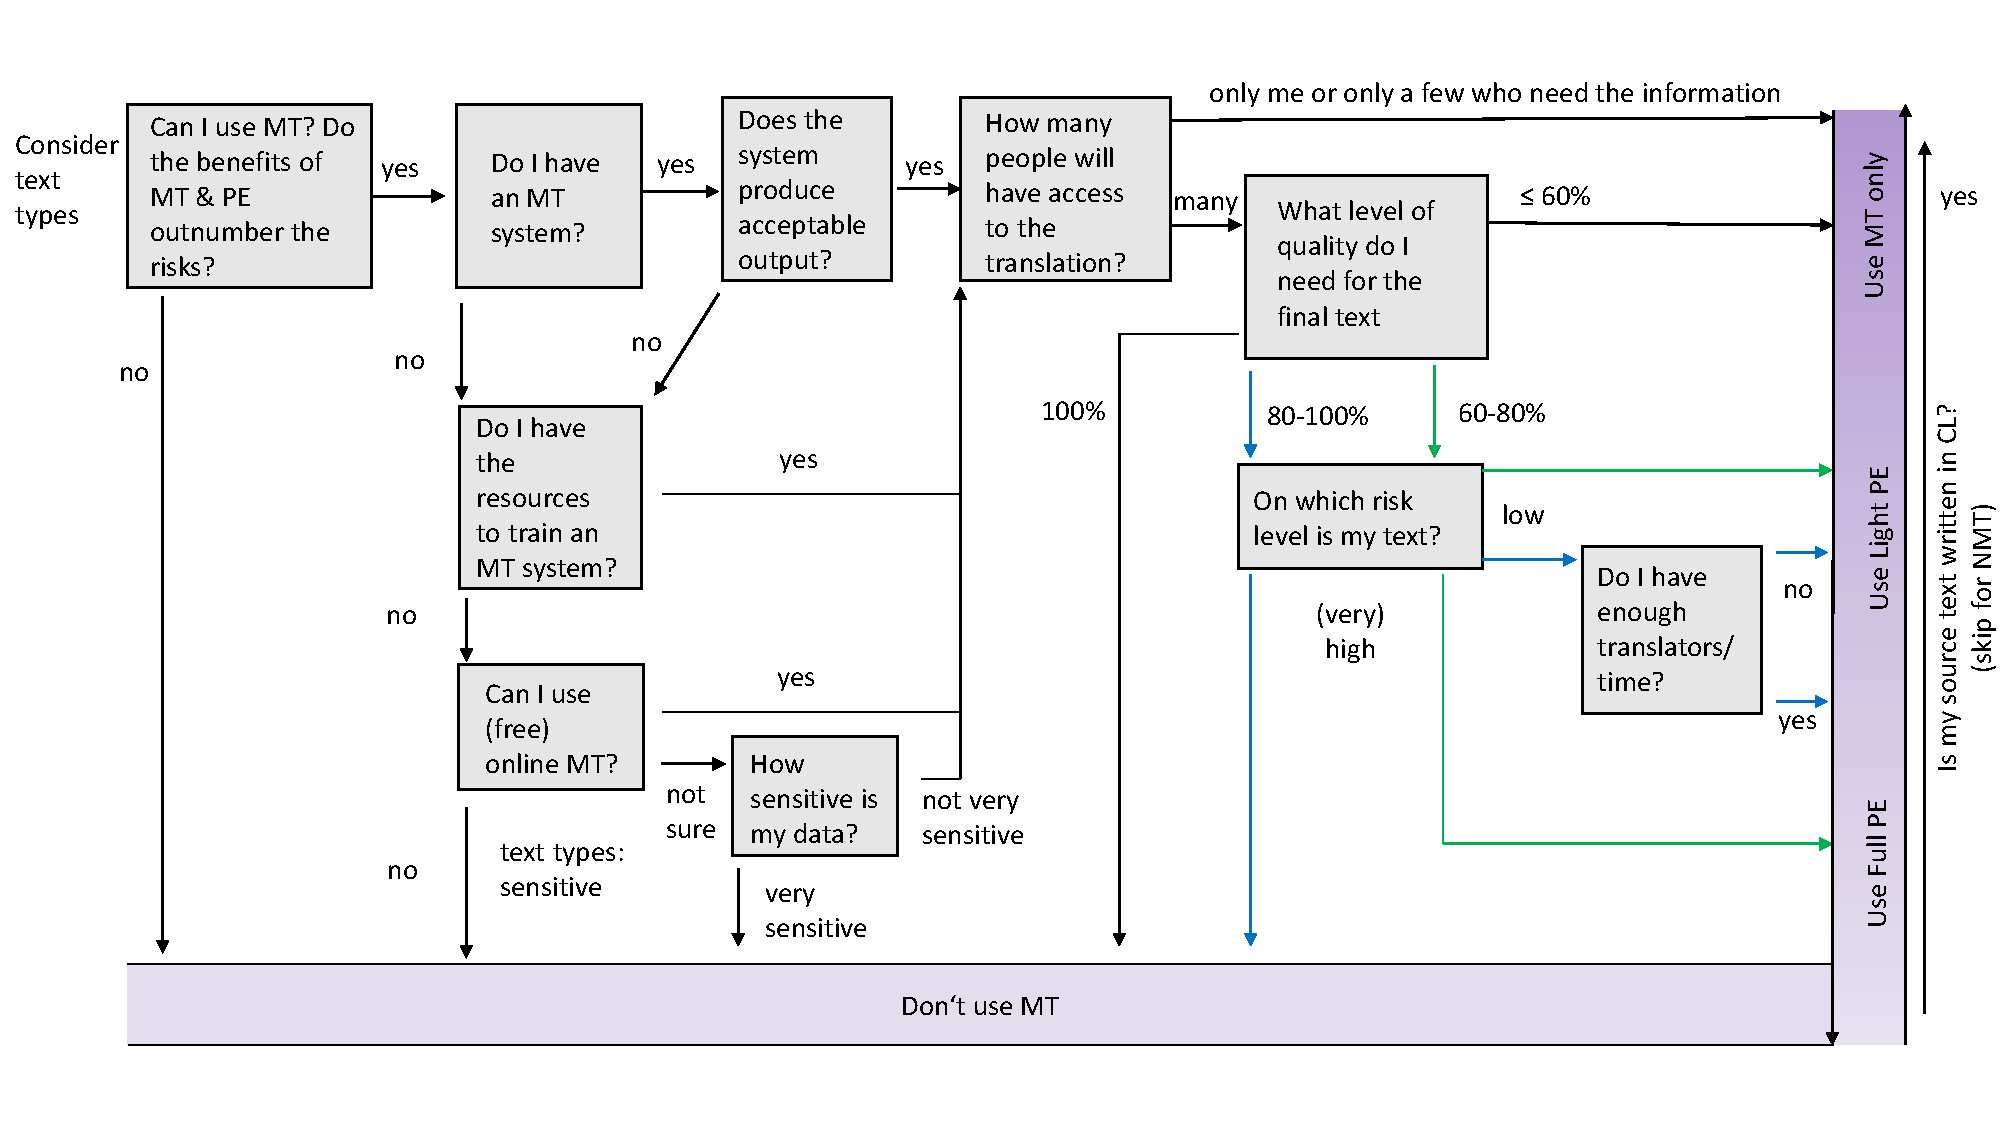
\includegraphics[width=\textwidth]{figures/art_nitzke_fig1.pdf}
\caption{Decision tree as in \citet[246]{nitzke2019risk}}
\label{fig:key:8:7}
\end{sidewaysfigure}

\citet{hor_chancen_2020} applied the decisions to the perspective of a language service pro\-vid\-er. She suggests that not all project managers should make decisions about PE projects, but only those who have PE experience. Another scenario could be that there is one (or more) designated PE expert(s). Further, she proposes to include a step for expectation management and pricing in the model -- the latter referring to the aspect that the amount of money put into the project guides the extent of the PE effort.

\newpage

\section*{Crossword puzzle -- Chapter 8}

\begin{Puzzle}{13}{14}
|{}	|{}	|{}	|{}	|{}	|{}	|{}	|{}	|{}	|{}	|[4]D	|{}	|{}	|.
|{}	|{}	|[1]P	|R	|E	|P	|A	|R	|A	|T	|I	|O	|N	|.
|{}	|{}	|{}	|{}	|{}	|{}	|{}	|{}	|{}	|{}	|S	|{}	|{}	|.
|{}	|{}	|{}	|{}	|{}	|[2]R	|{}	|{}	|{}	|{}	|T	|{}	|{}	|.
|{}	|{}	|{}	|{}	|{}	|E	|{}	|{}	|{}	|{}	|A	|{}	|{}	|.
|{}	|{}	|[5]D	|{}	|{}	|v	|{}	|{}	|{}	|{}	|N	|{}	|{}	|.
|{}	|[3]S	|E	|N	|S	|I	|T	|I	|V	|I	|T	|Y	|{}	|.
|{}	|{}	|F	|{}	|{}	|S	|{}	|{}	|{}	|{}	|{}	|{}	|{}	|.
|[7]S	|P	|E	|L	|L	|I	|N	|G	|{}	|{}	|{}	|{}	|{}	|.
|{}	|{}	|C	|{}	|{}	|O	|{}	|{}	|{}	|{}	|{}	|{}	|{}	|.
|{}	|{}	|[8]T	|U	|R	|N	|A	|R	|O	|U	|N	|D	|{}	|.
|{}	|{}	|I	|{}	|{}	|{}	|{}	|{}	|{}	|{}	|{}	|{}	|{}	|.
|{}	|{}	|V	|{}	|{}	|{}	|{}	|{}	|{}	|{}	|{}	|{}	|{}	|.
|{}	|[6]R	|E	|A	|D	|A	|B	|I	|L	|I	|T	|Y	|{}	|.
\end{Puzzle}

\begin{PuzzleClues}{\textbf{Across}}
\Clue{1}{PREPARATION}{What are the three stages of the translation process according to \cite{hofmann2012prozessgestutztes}? translation ... , translation, and translation post-processing}
\Clue{3}{SENSITIVITY}{When we assess whether a source text is appropriate for MT and PE, what are the three criteria we have to watch out for? Suitability of the source text for MT, risks, and ... of information}
\Clue{6}{READABILITY}{When a text is written in a controlled language, what is improved for the target audience?}
\Clue{7}{SPELLING}{What kind of mistakes in the source text might be corrected automatically?}
\Clue{8}{TURNAROUND}{What temporal aspect might cause very tight deadlines and might be a reason for PE, but should not still not outweigh quality considerations? ... time}
\end{PuzzleClues}

\begin{PuzzleClues}{\textbf{Down}}
\Clue{2}{REVISION}{What do we call the quality assurance step after a text has been fully post-edited or translated?}
\Clue{4}{DISTANT}{What kind of languages tend to be more difficult for MT because they are usually less linear? }
\Clue{5}{DEFECTIVE}{The source text decreases the quality of the MT output when it is very complex, very inconsistent, or ....}
\end{PuzzleClues}
